\documentclass[a4paper,11pt]{report}

\usepackage{fixltx2e}
\usepackage[english,frenchb]{babel}
\addto\captionsfrenchb{%
  \renewcommand{\listalgorithmname}{Algorithmes}%
}
\usepackage[utf8]{inputenc}
\usepackage[T1]{fontenc}
\usepackage{lmodern}
%\usepackage{helvet}
%\renewcommand{\familydefault}{\sfdefault}

\usepackage{microtype}

\usepackage{float}
\usepackage{graphicx}
\usepackage{wrapfig}
\usepackage{subcaption}

%\usepackage[a4paper]{geometry}  %PAPER VERSION
%\setlength{\textheight}{650pt}

\usepackage{multirow}

\usepackage[chapter]{algorithm}
\usepackage{algorithmic}
\algsetup{linenodelimiter=}
\renewcommand{\algorithmiccomment}[1]{\hfill$\triangleright$\textit{#1}}

\usepackage{amsmath}
\usepackage{amssymb}

\usepackage{listings}
\lstset{defaultdialect=[5.2]Lua, style=Lua, frame=single}

\usepackage{perpage}
\MakePerPage{footnote}

\pagestyle{headings}

\usepackage{ifthen}
\usepackage[title,titletoc]{appendix}
\newcommand{\appsec}[2][]{\clearpage%
\ifthenelse{\equal{#1}{} }{
  \section{#2}
}{
  \section[#1]{#2}
}}
%syntax is:
%\begin{subappendices}
%  \appsec[short title]{appendix title}
%\end{subappendices}

\bibliographystyle{myAlphaurl}

\usepackage[colorlinks=true,linktoc=page]{hyperref}

\usepackage[symbol=$^{\blacktriangle}$]{footnotebackref}

\newcommand{\HRule}{\rule{\linewidth}{0.5mm}}

\usepackage{tikz}
\usetikzlibrary{shapes,arrows}


\title{Robot en essaim: explorez}
\author{Sacha Alcalde Mangen, Shankar Baba, Rosine Desmet, Nathan Dwek, Bernard Gonda}

\begin{document}

\begin{titlepage}
\begin{center}

% Upper part of the page. The '~' is needed because \\
% only works if a paragraph has started.

\includegraphics[width=0.4\textwidth]{EPB.jpg}~\\[1cm]

\textsc{\LARGE Ecole Polytechnique de Bruxelles\\Université Libre de Bruxelles}\\[1.5cm]

\textsc{\Large Rapport du projet de Ba2: Groupe 9}\\[0.5cm]

% Title
\HRule \\[0.4cm]
{ \huge \bfseries Robots en Essaim: Explorez\\[0.4cm] }

\HRule \\[1.5cm]

% Author and supervisor
\begin{minipage}{0.4\textwidth}
\begin{flushleft} \large
\emph{Etudiants:}\\
Sacha \textsc{Alcalde Mangen}\\
Shankar \textsc{Baba}\\
Rosine \textsc{Desmet}\\
Nathan \textsc{Dwek}\\
Bernard \textsc{Gonda}\\
\end{flushleft}
\end{minipage}
\begin{minipage}{0.4\textwidth}
\begin{flushright} \large
\emph{Superviseur:} \\
Ir. Anh Vu \textsc{Doan Nguyen}
\end{flushright}
\end{minipage}

\vfill

% Bottom of the page
{\large \today}

\end{center}
\end{titlepage}

\selectlanguage{english}
\begin{abstract}
The goal of this project was to design a swarm-intelligent behaviour for virtual robots using the ARGoS software. These robots had to explore an unknown environment with obstacles in order to ultimately loop between spots marked on the ground and a starting area. The fundamental paradigm was that a single set of rules would be followed independently by every robot, which would allow a swarm-intelligent behaviour to emerge through the robot interactions prescribed by these rules. For that to work, exploration, shortest path-finding and obstacle-avoidance algorithms were needed, along with elementary automated decision making, communication and odometry. These concepts were implemented using the ARGoS loop approach, which means that the same sequence of actions takes place at every step, while only events occurring during that step can influence these actions. A working solution was produced using the Lua language, then put to the test and could quickly be enhanced accordingly thanks to the flexible framework. This allowed robots to meet the objectives and information was gathered on parameters meaningful for the experiment along with performance indexes. Future development should be focused on optimizing these parameters and enable the footbots with the latest advances in swarm intelligence, like the usage of simulated pheromones, for example.

\end{abstract}

\selectlanguage{frenchb}
\begin{abstract}
Le but de ce projet était de créer une intelligence en essaim pour des robots modélisés dans le simulateur ARGoS. Ceux-ci devaient explorer un environnement inconnu qui comportait des obstacles afin d'ensuite faire des allers-retours entre des zones marquées aux sols et leur nid de départ. Le principe de base était que le même ensemble de règles devrait être suivi de manière indépendante par chaque robot; la caractéristique intelligente de l'ensemble de robots devant émerger à travers les interactions entre robots prescrites par ces règles. Pour cela, des procédures d'exploration, de recherche du plus court chemin et d'évitement furent nécessaires ainsi que des principes de base de prise de décision, d'odométrie et de communication. Ces concepts furent mis en pratique en utilisant l'approche loop d'ARGoS, qui implique que le robot exécute la même séquence d'opérations à chaque pas. Une solution fonctionnelle en Lua fut construite, testée et ensuite améliorée en conséquence grâce au turnaround loop très court offert par ARGoS. Cette solution permet aujourd'hui au robots de remplir les objectifs, et des informations ont été collectées sur des paramètres influençant l'expérience, ainsi que des indicateurs de performances. Des développements futurs pourraient être consacrés à l'optimisation de cette solution et à utiliser les dernières trouvailles de l'intelligence en essaim, comme par exemple les phéromones-messages artificielles, dans le comportement des footbots.

\end{abstract}

\tableofcontents

\chapter{Introduction}
Le but du projet est de doter un essaim de robots d'un comportement intelligent afin qu'ils soient capables \cite{cahierCharges}
\begin{itemize}
  \item d'explorer un environnement inconnu afin de localiser des <<sources>> symbolisées par des taches noires au sol
  \item d'<<exploiter>> les sources découvertes en faisant des allers-retours entre celles-ci et le nid
  \item de partager l'information accumulée afin d'optimiser l'exploitation des sources
  \item d'accomplir ces tâches dans un environnement comportant des obstacles, tout en gérant leur autonomie limitée
\end{itemize}
L'essaim de robots et son environnement sont simulés par ARGoS, un simulateur développé par le laboratoire IRIDIA.

\section{Intérêt du projet}

Comme son nom l'indique, la robotique en essaim met en oeuvre un nombre élevé de robots afin d'effectuer une tâche. Ceci est très différent de ce qui se fait habituellement en robotique <<classique>> où un petit nombre de robots extrèmement sophistiqués est déployé afin de résoudre une problématique. Les principes fondamentaux derrière la programmation d'un essaim de robots peu coûteux mais au capacités plus limitées sont donc aussi différents: chaque individu ne doit plus être considéré comme infaillible, et la perte d'un robot prend moins d'importance, tant qu'elle profite à l'essaim tout entier. Ceci ouvre de nouvelles voies dans de nombreux domaines, par exemple dans le cas très concret du déminage ou lorsqu'il faut opérer dans une zone hautement hostile au sens plus général (intervention en milieu radioactif, en grande profondeur, \ldots).~\cite{swarmMini}

\section{Résultats attendus}

L'objectif premier est de développer un comportement qui permet aux robots de survivre et d'exploiter une ressource de manière autonome dans un environnement non connu à l'avance.

Dans un premier temps, les robots seront considérés comme omniscients et connaîtront donc l'environnement à explorer. Cette connaissance leur sera ensuite retirée. Une communication entre les robots pourra être envisagée par la suite et permettra nottament de mieux gérer l'information incomplète.

Même si la tâche à accomplir est au niveau de l'essaim, ce dernier ne sera jamais programmé directement. Le principe même du projet est de développer un comportement qui sera suivi par chaque robot indépendamment. Des interactions locales entre robots, physiques ou non, émergera un comportement global qui devra être étudié et être rendu prévisible.

Des outils de mesure, afin de calculer la qualité du comportement en essaim, devront être élaborés. Ils devront établir la performance des solutions proposées en fonction des objectifs initiaux.~\cite{cahierCharges}

\vspace{1em}Ce rapport a été divisé en trois parties: une introduction à la notion d'intelligence artificielle et de comportement en essaim en particulier, la problématique du déplacement des robots et enfin la mise en place à un niveau plus haut d'un comportement <<intelligent>> permettant de remplir les objectifs décrits plus haut.

\chapter{L'intelligence artificielle\label{chap:AI}}
PROBABLEMENT BESOIN D'UN PETIT PEU DE REECRITURE ICI

Afin de mener à bien l'objectif énoncé dans l'introduction, les robots doivent se comporter de manière intelligente. Le plus important est l'interaction avec l'environnement. En effet, le choix de la bonne action est cruciale. Il est cependant délicat de définir une seule <<meilleure>> action. Ceci est développé plus bas, en introduisant le concept de \emph{rationalité}.
De manière générale, un robot peut être assimilé à un agent qui reçoit des \emph{percepts} par l'intermédiaire de ses capteurs. L' \emph{agent} réagit alors en exerçant une action sur l'environnement grâce à ses \emph{effecteurs}.
\begin{figure}[htb]
  \centering
  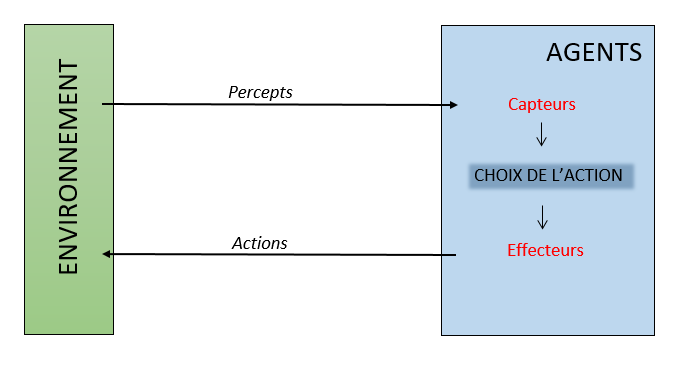
\includegraphics[width=0.9\textwidth]{pics/cycleInteractionAI.png}
    \caption{Cycle d'interaction entre l'environnement et les agents}
\end{figure}
La description des différents capteurs et effecteurs du robot est faite dans le chapitre \ref{chap:argosFootbot}.

Comme énoncé précédemment la rationalité d'un agent peut être délicate à mesurer. D'après \cite{AIBrique}:
\begin{quote}
  <<La rationalité n'est pas synonyme de perfection, la rationalité maximise la performance espérée tandis que la perfection maximise la performance réelle.>>
\end{quote}


En effet, dans un groupe composé de plusieurs agents, un choix d'action peut s'avérer bénéfique pour un agent mais mauvais pour l'ensemble du groupe. C'est pourquoi il est préférable de concevoir les mesures de performance en fonction de ce que l'on souhaite obtenir dans l'environnement et non en fonction de la façon dont devrait se comporter un agent.

A partir de cela, tout problème peut être formellement défini par cinq composantes. Tout d'abord l'état initial dans lequel commence l'agent, puis la description de ses différentes actions, c'est à dire toutes les actions possibles dans un état donné. Ensuite, vient le modèle de transition, il décrit ce que chaque action réalise. Ces trois premières composantes définissent l'espace des états du système, c'est à dire l'ensemble de tous les états accessibles par une séquence d'action à partir de l'état initial.

Dès lors l'espace d'état peut être interprété sous forme d'arbre où les nœuds représentent des états et les branches des séquences d'action. Il en découle la notion de chemin représentant une séquence d'états reliés par une séquence d'action.

La quatrième composante correspond au test but. Celle-ci détermine si un état donné est un état but. Enfin vient la cinquième et dernière composante, le coût du chemin. Elle permet d'attribuer une valeur numérique à un chemin en accord avec la mesure de performance imposée.

Maintenant qu'une présentation générale de l'intelligence artificielle a été faite, le comportement d'essaim d'agents intelligents peut être étudié. Pour ce faire, il s'est avéré très intéressant d'en comprendre le comportement à partir d'exemples se trouvant dans la nature. Les fourmis et les abeilles illustrent bien cela. Deux algorithmes mettant en avant leur comportement sont présentés ci-dessous.

\section{Algorithme des fourmis}

TODO/TO RETHINK +CF SECTION 4.6.2

OLD:
Cet algorithme est basé sur le comportement des fourmis dont une des particularités est la communication au travers de l'environnement par dépôts de phéromones.

L'algorithme se présente de la manière suivante. Pour commencer, une exploration de l'environnement est faite par les fourmis. Si l'une d'entre elles trouve une source, elle déposera, lors de son retour au nid, des phéromones tout au long du chemin qu'elle emprunte. Dès lors, lorsque que d'autres fourmis partiront à la recherche de nourriture, elles auront tendance à suivre le chemin  marqué de phéromones. Et à leur retour à la colonie, elles renforceront cette piste.

Cet algorithme illustre une communication indirecte d'un essaim et la manière dont ce dernier est influencé \cite{antOpti}. L'autre algorithme, illustrant le comportement d'une structure organisée, est l'algorithme des abeilles.


\chapter[ARGoS et les footbots]{Présentation du simulateur ARGoS et des footbots\label{chap:argosFootbot}}
\section{Capteurs et actuateurs des footbots}

Comme présenté plus haut, les capteurs et actuateurs des agents déterminent bien évidemment les informations qu'ils sont capables de recueillir et les actions qu'ils peuvent effectuer.

\begin{figure}[htb]
  \centering
  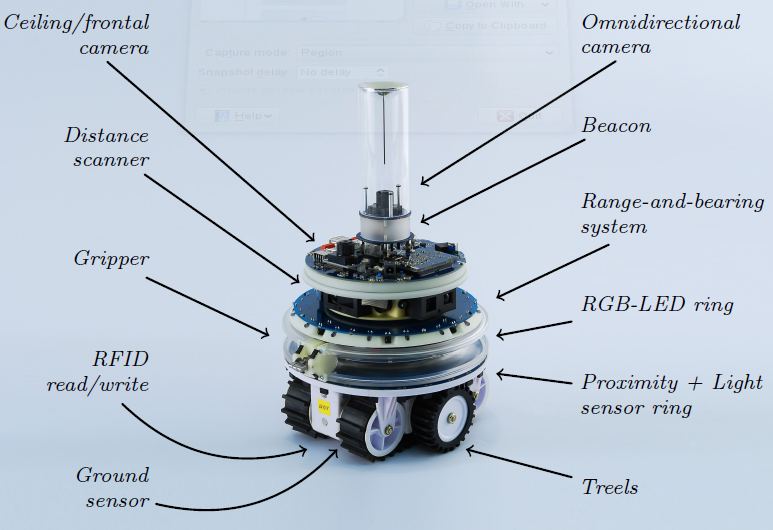
\includegraphics[width=0.9\textwidth]{pics/footbot.png}
  \caption{Les différents senseurs et actuateurs d'un footbot~\cite{argosSite1}}
\end{figure}

Dans le cadre du projet, on considère qu'il suffit que le robot passe sur une <<source>> pour l'exploiter. Les différents capteurs et actuateurs intéressants sont alors les roues, le senseur de proximité et le \emph{distance scanner} pour la partie déplacement, le \emph{ground sensor} pour la partie exploration (car il permet de lire la couleur du sol), et enfin les différentes LED et le système \emph{range and bearing} ainsi que les capteurs associés pour la partie communication.

Comme annoncé dans l'introduction, l'essaim de robots devra être simulé dans ARGoS, un simulateur de robots développé notamment par le département IRIDIA de l'ULB. Ce simulateur a besoin de deux fichiers pour lancer une expérience: un fichier XML qui permet de configurer l'arène et l'expérience en général (moteur physique, capteurs et actuateurs disponibles, \ldots) \cite{argosReport} d'une part, et un fichier dictant le (même) comportement individuel de chaque robot d'autre part. Pour l'instant, les instructions peuvent être écrites soit en C++, soit en Lua.


\section{Choix du langage informatique}

D'une part, les principaux avantages de C++, sa rapidité d'exécution et ses nombreuses librairies notamment, ne sont pas primordiaux dans le cadre de ce projet. De plus, il nous est moins familier que Lua qui se rapproche fortement de python tant au niveau de la syntaxe que de l'approche fonctionnelle.

Lua étant un langage de scripting, il est plus adapté aux besoins du groupe car la réalisation du projet passe par de nombreuses petites expérimentations mais ne devrait pas aboutir à un comportement final comportant de très nombreuses lignes de code. En effet, ce type de langage permet de concevoir des prototypes de programmes rapidement.

Enfin sa simplicité et sa lisibilité sont des aspects très importants dans un travail de groupe où chacun doit être capable de comprendre et d'améliorer le comportement en développement.~\cite{compC++,compLua}

Au vu des raisons énoncées ci-dessus, Lua a été choisi comme langage de programmation.

\section{Structure d'un comportement en Lua}

Le template de code fourni par ARGoS présenté plus bas montre les deux fonctions les plus importantes parmi les fonctions que le simulateur doit absolument trouver dans le comportement. La fonction \emph{init} qui est exécutée une fois par chaque footbot au début de l'expérience, et la fonction \emph{step} qui est exécutée par chaque footbot à chaque pas de la simulation. C'est bien évidemment cette fonction \emph{step} qui représente presqu'entièrement le comportement du robot. Deux types d'évènements peuvent modifier la façon dont cette fonction step s'exécute: d'une part, les percepts ayant lieu au cours du pas de simulation, et d'autre part un ensemble de variables globales (qui survivent après l'exécution de la fonction \emph{step} et sont donc accessibles par les instances suivante de cette fonction) qui détermine entièrement l'état du robot lorsque celui-ci entame ce pas de simulation. Enfin, la fonction step peut agir en retour sur ces variables d'état.~\cite{argosSite1}
\begin{lstlisting}[caption=Structure de base d'un comportement en Lua]
--[[ This function is executed every time
     you press the 'execute' button ]]
function init()

end

--[[ This function is executed at each time step
     It must contain the logic of your controller ]]
function step()

end
\end{lstlisting}

\section{Configuration de l'arène et de l'expérience}

L'arène a aussi dû être créée par le groupe selon les spécifications données:
\begin{itemize}
  \item L'arène est carrée de côté 10m
  \item Le nid et les sources font 50cm de rayon
  \item L'arène comporte éventuellement des obstacles
  \item Les robots ont une batterie de 100 et perdent 0.2 par pas\footnote{Ceci impose une vitesse $>25cms^{-1}$ afin que les foobots puissent raisonnablement faire des allers-retours vers les coins de l'arène, ce qui est largement supérieur à la vitesse de $10cms^{-1}$ utilisée dans des travaux précédents \cite{foraging, pheromonesForaging}.}
  \item Les robots récupèrent leur batterie en passant par le nid
\end{itemize}

L'arène utilisée comporte entre 50 et 100 obstacles cylindriques de 10cm de rayon disposés au hasard. Différentes répartitions de ressources ont été envisagées. De plus, un script python a été utilisé pour mettre en place aléatoirement de nombreuses expériences et automatiser la collecte de données. Une configuration initiale typique est montrée à la figure \ref{fig:initArena}.
\begin{figure}[htb]
  \centering
  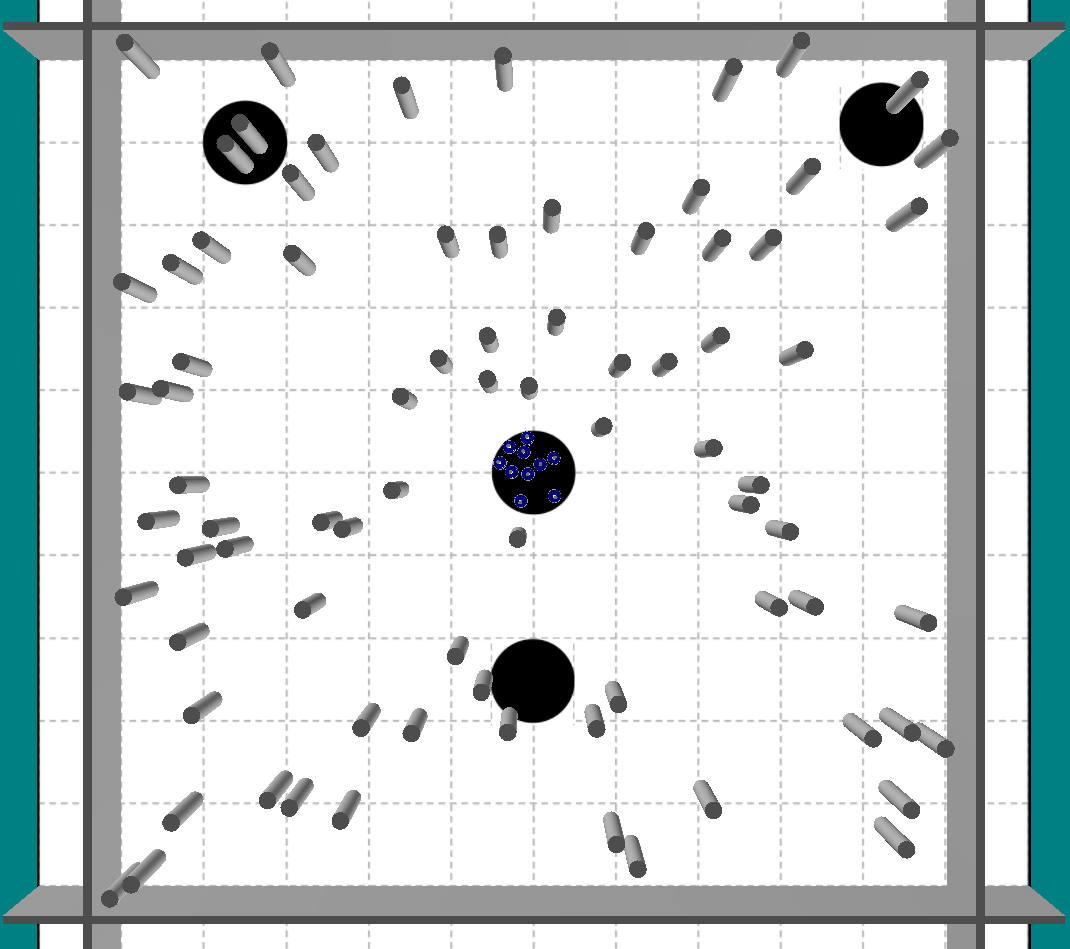
\includegraphics[width=0.9\textwidth]{pics/initArena.png}
  \caption{Exemple de configuration initiale\label{fig:initArena}}
\end{figure}




\chapter{Déplacement et évitement d'obstacles \label{chap:move}}
Comme il a été présenté dans l'introduction sur l'intelligence artificielle, et vu en pratique dans la structure de base d'un comportement Lua interprétable par ARGoS, un footbot exécute à chaque step une séquence d'opérations. On peut distinguer dans cette séquence trois types d'opérations (cf chapitre \ref{chap:AI}): l'écoute des capteurs, la prise de décision et les interactions sur l'environnement par l'intermédiaire des effecteurs, que l'on nommera ici simplement sous le nom d'actions. Ces actions sont donc limitées et déterminées par les effecteurs dont dispose le robot et qui sont décrits au chapitre \ref{chap:argosFootbot}. Dans ce chapitre-ci, l'un des effecteurs primordiaux d'un footbot sera examiné: son déplacement.

\section{Aspects physiques du déplacement}

Tout d'abord, il est intéressant de se pencher sur le lien entre les paramètres physiques du robot et la manière dont celui-ci peut effectuer l'action simple «se rendre d'un point A à un point B» dans le cas où le robot agit seul dans un environnement sans obstacles. Ensuite, nous verrons comment le robot peut s’accommoder des obstacles (fixes, prévisibles) et autres robots (mobiles, imprévisibles) à partir d'une ou plusieurs de ces actions simples.

\begin{wrapfigure}{r}{0.3\textwidth}
  \vspace{-3em}
  \begin{center}
    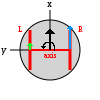
\includegraphics[width=0.15\textwidth]{pics/robotWheels.png}
  \end{center}
  \vspace{-2em}
  \caption{Signification physique de \(v_r,\: v_l,\: v_g \; et \; \omega_g \) \cite{argosSite1}}
  \vspace{-1em}
  \end{wrapfigure}
L'effecteur dont un footbot dispose afin de se déplacer est une paire de roues dont les vitesses peuvent être fixées de manière indépendante. A chaque instant, les seuls deux mouvements auxquels peut accéder le robot sont donc une translation parallèle aux roues et une rotation autour d'un point au milieu de l'axe des roues. La mécanique~\cite{meca} nous indique que la composition de ces deux mouvements est suffisante pour permettre au robot de se déplacer librement dans un plan mais surtout, elle nous donne la relation entre les vitesses des deux roues et la vitesse générale ainsi que la vitesse de rotation du robot:
\begin{equation}
\begin{cases}
v_g=\frac{v_r+v_l}{2}\\
\omega_g=\frac{v_r-v_l}{l_{axe}}
\end{cases}
\end{equation}

\section{Déplacement sans obstacles}

A partir de cette loi des vitesses, il est aisé de construire un algorithme permettant à un robot de converger vers sont but selon une trajectoire souple et à vitesse constante.

\begin{algorithm}
\caption{Convergence with no obstacle avoidance}
\label{simpleConvergence}
\begin{algorithmic}
  \REQUIRE \(SPEED \equiv \) Fixed speed of the footbot \(> 0\)
  \REQUIRE Goal in arena
  \ENSURE footbot converges towards the goal at speed \(SPEED\)
  \WHILE{goal not reached}
    \STATE update footbot position and orientation
    \STATE calculate \( \theta \equiv\) angle between the direction of the goal from the footbot and footbot orientation
    \STATE \( right\:velocity \gets\) convergence(\(\theta,\:SPEED\))
    \STATE \( left\:velocity \gets 2 \times SPEED-right\:velocity\) \COMMENT{so that overall speed stays equal to SPEED}
  \ENDWHILE
\end{algorithmic}
\end{algorithm}

Où convergence($\theta, SPEED$) fixe la convergence du robot vers son goal. Elle doit satisfaire:

\begin{equation}
  \begin{cases}
    convergence(0,SPEED)=SPEED\\
    convergence(\overset{\text{goal à gauche du robot}}{\overbrace{0<\theta\leq\pi}},SPEED)>SPEED\\
    convergence(\overset{\text{goal à droite du robot}}{\overbrace{0>\theta\geq-\pi}},SPEED)<SPEED
  \end{cases}
\end{equation}

Pour une fonction convergence($\theta, SPEED$) donnée satisfaisant à cette condition (par exemple dépendance linéaire en \(\theta\)), le footbot peut donc se rendre d'un point A à un point B, tant qu'il ne rencontre pas d'obstacles sur son trajet. Notons que cet algorithme s'intègre particulièrement bien dans la fonction \emph{step} demandée par ARGoS. Dans notre projet nous avons choisi
\[
convergence(\theta, SPEED)=
\begin{cases}
      { \left( \frac{\pi- \lvert \theta \rvert }{\pi} \right)}^{\kappa} \times SPEED & \text{si } \theta \geq 0\\
      \left( 2 - { \left( \frac{\pi- \lvert \theta \rvert }{\pi} \right) }^{\kappa} \right) \times SPEED & \text{si } \theta < 0
\end{cases}
\]
Où $\kappa > 0$ est un paramètre qui fixe l'intensité de la convergence.

\section{Évitement \emph{greedy} d'obstacles lointains}

Une première manière de permettre au robot d'éviter des obstacles est d'activer le capteur \emph{distance scanner} longue distance qui permet de détecter des obstacles jusqu'à 150cm du footbot. Un évitement très efficace mais parfois trop gourmand consiste alors à chercher à chaque pas la direction la plus proche de la direction du goal et pour laquelle l'obstacle repéré est le plus éloigné du robot (ou non existant) et à converger vers celle-ci. Ceci permet au robot d'éviter plusieurs obstacles à la fois, tout en gardant une trajectoire très optimisée.

\begin{algorithm}
\caption{Convergence with greedy obstacle avoidance}
\label{greedyConvergence}
\begin{algorithmic}
  \WHILE{goal not reached}
    \STATE update footbot position and orientation
    \STATE find \( \theta \equiv\) angle between footbot orientation and best direction (closest to goal, least obstacles)
    \STATE \( right\:velocity \gets\) convergence(\(\theta,\:SPEED\))
    \STATE \( left\:velocity \gets 2 \times SPEED-right\:velocity\) \COMMENT{so that overall speed stays equal to SPEED}
  \ENDWHILE
\end{algorithmic}
\end{algorithm}

La fonction convergence doit satisfaire au mêmes contraintes que précédemment et reste inchangée dans notre projet. Pour que l'évitement soit efficace, il faut que $\kappa$ soit assez élevé pour que le footbot s'oriente rapidement vers la direction optimale. Malgré cela, cet évitement reste très \emph{greedy}, dans le sens ou chercher absolument la direction la plus proche de celle du but peut mener à des collisions à cause de différents facteurs et approximations (footbot de taille non nulle, rayons du \emph{distance scanner} parfaitement tangent à un obstacle, \emph{distance scanner} ne faisant pas une mesure par direction à chaque pas, nombre de directions mesurées bien évidemment fini, \ldots). Une première manière de pallier à cela est de regrouper plusieurs mesures voisines en gardant systématiquement la mesure la moins optimiste. Magré cela, un évitement plus sûr d'obstacles proches est aussi nécessaire pour limiter le plus possible les collisions.

Cet évitement d'obstacles est directement utilisé dans notre projet. Son implémentation est détaillée dans l'annexe \ref{app:implEvitGreedy}

\section{Evitement sûr d'obstacles proches\label{sec:emerAvoid}}

La manière la plus directe de permettre au footbot d'éviter des obstacles ou autres robots lorqu'ils sont dangereusement proches est d'alors exécuter une routine d'évitement à la place de la routine de convergence précédente.
\begin{algorithm}
\label{obstacleConvergence}
\caption{Convergence with close obstacle avoidance}
\begin{algorithmic}
  \ENSURE footbot converges towards the goal at speed \(SPEED\) while avoiding obstacles
  \WHILE{goal not reached}
    \STATE update footbot position and orientation
    \STATE read proximity sensors \COMMENT{or whatever other sensor in use}
    \IF{no obstacles too close}
      \STATE do previous convergence
    \ELSE
      \STATE \( right\:velocity \leftarrow\) avoidance(proximity sensor reading, \(SPEED\))
    \ENDIF
    \STATE \( left\:velocity \leftarrow 2 \times SPEED-right\:velocity\) \COMMENT{so that overall speed stays equal to SPEED}
  \ENDWHILE
\end{algorithmic}
\end{algorithm}

Où avoidance(proximity sensor reading, $SPEED$) fixe la routine d'évitement du robot. Son implémentation est très libre et peut fortement varier en fonction du capteur utilisé pour détecter les obstacles. On peut par exemple utiliser le senseur \emph{proximity} du footbot, qui associe à 24 directions autour du robot une valeur entre zéro et un: une valeur zéro indique qu'aucun obstacle n'est perçu à moins de 10cm dans la direction donnée tandis qu'une valeur supérieure indique qu'un objet a été détecté. Cette valeur augmente au fur et à mesure que le robot se rapproche de l'obstacle.~\cite{argosSite1}

Dans notre projet nous avons choisi
\[avoidance(dir, prox)=
  \begin{cases}
      \frac{-\alpha +(1-prox)^{\beta}\cdot dir}{11}SPEED & \text{si }dir \leq 12\\
      \frac{(22+\alpha )-(1-prox)^{\beta}\cdot (25-dir)}{11}SPEED & \text{si }dir \geq 12\\
  \end{cases}
\]

Où $ 1 \leq dir \leq 12 $ est la direction de l'obstacle perçu le plus proche et \hbox{$0 \leq prox \leq 1$} donne la proximité de cette obstacle. Comme présenté plus haut, ce sont les deux informations dont on dispose si l'on utilise le capteur de proximité.  \(1 \leq \alpha \leq 12 \) est un paramètre qui fixe l'influence de la direction de l'obstacle le plus proche et \(0 \leq \beta \) fixe l'influence de la proximité de cette obstacle. Cet évitement est partiellement tiré des exemples fourni sur le site du cours présentant ARGoS \cite{argosSite1}.

\section{Evitement intermédiaire}

Additionnellement, il est possible d'utiliser le capteur \emph{short range} du \emph{distance scanner} pour que le robot puisse déjà commencer à dévier sa trajectoire s'il détecte des obstacles proche de moins de 30cm~\cite{argosSite1}. Ceci permet de déclencher plus tôt le même évitement aux constantes numériques près (évitement moins brusque) que ci-dessus. Cet évitement est beaucoup moins \emph{greedy} que le premier évitement présenté, tout en étant forcément plus souple que l'évitement <<d'urgence>> précédent.

De plus, les capteurs \emph{short range} et \emph{long range} sont des capteurs rotatifs, ce qui signifie que la table des mesures n'est pas complètement renouvelée à chaque pas\footnote{D'où la nécessité de rafraîchir les tables de mesures de la manière qui est faite au listing \ref{lst:updateObstaclesTable}}. Les deux capteurs étant orientés perpendiculairement, il est donc avantageux de les utiliser tous les deux afin de ne pas avoir de direction pour laquelle la dernière mesure est <<trop vieille>>.

Grâce à aux différentes routines élémentaires présentées ci-dessus, il est donc possible de construire une résoudre la partie déplacement du cahier des charges. L'implémentation détaillée des routines d'évitement supplémentaire est donnée dans l'annexe~\ref{app:implEvitClose}

\section{Déplacement selon un chemin précalculé}

Il est cependant possible d'améliorer cette solution en fonction de la connaissance de son environnement dont dispose le robot. Ainsi, dans le cas omniscient ou si le robot est capable de construire une carte de son environnement reprenant la position des différents obstacles il peut-être judicieux d'utiliser un algorithme de recherche du plus court chemin. La manière la plus directe de faire est de donner au footbot une liste de goal successifs qui le mèneront au goal final. Ceci  permet de réutiliser facilement les algorithmes déjà présentés tout en étant parfaitement compatible avec les valeurs de retour typiques d'un algorithme de recherche du plus court chemin. En effet, la plupart des recherches du plus court chemin utilisent une représentation en graphe d'un environnement. La valeur de retour d'une telle recherche est donc une liste des nœuds qu'il faut parcourir dans le graphe afin d'arriver au but final, ce qui est précisément ce que cet algorithme fait.
\begin{algorithm}
\caption{Convergence with path finding}
\label{pathConvergence}
\begin{algorithmic}
  \REQUIRE intermediate goals list $\equiv$ list of points which lead to the goal while avoiding the obstacles
  \ENSURE footbot goes to goal while avoiding obstacles
  \FOR{intermediate goal in intermediate goals list}
  \WHILE{intermediate goal not reached}
    \STATE update footbot position and orientation
    \STATE read proximity sensors \COMMENT{or whatever other sensor in use}
    \IF{no obstacles too close}
      \STATE do greedy avoidance
    \ELSE
      \STATE do close obstacle avoidance
    \ENDIF
  \ENDWHILE
  \ENDFOR
\end{algorithmic}
\end{algorithm}

L'implémentation de l'algorithme de recherche du plus court chemin qui fournit intermediate goals list est un problème à part entière. Avant de l'examiner plus en détail, il faut noter que malgré l'utilisation d'une recherche du plus court chemin qui devrait a priori permettre d'éviter les obstacles, le test d'obstacle est toujours présent, ainsi que la possibilité d'évitement. Il est évident que ceci est fait pour permettre d'éviter des objets inattendus tels que d'autres robots, par exemple. Cependant, on peut dès lors se demander s'il ne faudrait pas aussi chercher de nouveau un plus court chemin après un évitement imprévu ou si le robot a dévié d'une distance significative de sa trajectoire prévue.

\subsection{Recherche du plus court chemin}

\subsubsection{Algorithme A*}
\cite{wikiA*}

En informatique, A* est un algorithme informatique qui consiste à mettre en place un processus de traçage d'un chemin traversable efficace entre des points. Les points sont considérés comme des noeuds.

A* utilise une «best-first» recherche et trouve le chemin possédant le moindre coût à partir d'un nœud initial donné à un nœud but.

Pour cela, il utilise une fonction de coût pour déterminer l'ordre dans lequel les visites de recherche des nœuds de l'arbre vont s'effectuer. Cette fonction de coût est la somme de deux autres fonctions. La fonction coût de la trajectoire passée qui est la distance connue à partir du nœud de départ au dernier parcouru lors de la recherche. Et la fonction coût du chemin futur qui est une estimation heuristique de la distance entre le dernier nœud parcouru et le nouveau nœud à atteindre .

\begin{wrapfigure}{r}{0.3\textwidth}
  \vspace{-20pt}
  \begin{center}
    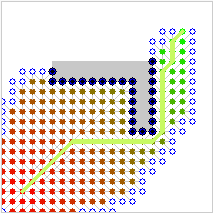
\includegraphics[width=0.28\textwidth]{pics/aStar.png}
  \end{center}
  \caption{Représentation d'une éxécution de A*\cite{wikiA*}}
\end{wrapfigure}
Cet algorithme possède quand même des limites. Il est effectivement efficace dans le cas où l'on considère les robots comme omniscient, connaissant l'environnement et, donc, connaissant la position de la source et des obstacles se trouvant dans l'environnement. Dans le cas de non-omniscience, l'arène est inconnue et on ne possède aucunes données à propos de celles-ci. Et c'est ici que se trouve le plus grand défaut de l'algorithme A*.

A* détermine un chemin complet de nœuds pour arriver d'un noeud départ à un noeud but. Lorsqu'il ne possède pas de données complètes à propos de l'arène, il est bloqué lors de son exécution et ne peut donc pas déterminer le chemin que doit suivre le robot. Il faudra adapter l'algorithme A* afin de remédier à ce problème.

\subsubsection{Algoritme de Dijkstra}
\cite{wikiDijkstra}

L’algorithme de Dijkstra est un algorithme servant à résoudre le problème du plus court chemin. Le principe de l'algorithme est le suivant:

Il s'agit de mettre en place progressivement un sous-graphe dans lequel sont classés les différents sommets. Un ordre croissant est établit entre les sommets et il est fixé en fonction de la distance minimale qui éloignent ces sommets à celui de départ. Cette distance correspond à la somme des nœuds parcourus.

Au début, les distances de chaque sommet par rapport au sommet de départ sont considérées comme infinie et on attribue à celui-ci une distance de 0.

Ensuite, au cours de chaque itération, les distances des sommets reliés par un nœud au dernier du sous-graphe sont mis à jour. Cette mis à jour consiste à ajouter la valeur du nœud à la distance séparant le sommet de départ à ce dernier sommet. Après cette mise à jour, l'ensemble des sommets, ne faisant pas partis du sous-graphe, sont examinés et celui qui possède la distance minimal y est ajouté.

Enfin, on répète l'exécution jusqu'à l'épuisement des sommets ou jusqu'à la sélection du sommet d'arrivée.
Voici 3 figures qui représentent un exemple du principe utilisé. Le but est de trouver le plus court chemin entre le point A et le point J. Comme dit précédemment, après chaque mise à jour, le sommet possédant la distance minimale est rajouté au sous graphe. La figure \ref{fig:dijkstra} représente bien cela.
\begin{figure}[h!]
        \centering
        \begin{subfigure}[h!]{0.4\textwidth}
                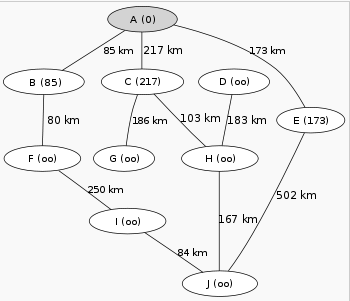
\includegraphics[width=\textwidth]{pics/dijk1.png}
                \caption{Mise à jour initiale\\\(\;\)}
        \end{subfigure}   \begin{subfigure}[h!]{0.4\textwidth}
                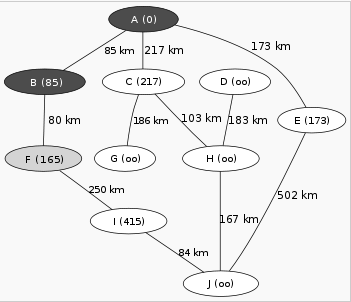
\includegraphics[width=\textwidth]{pics/dijk2.png}
                \caption{Mise à jour et construction du sous-graphe}
        \end{subfigure}

        \begin{subfigure}[h!]{0.4\textwidth}
                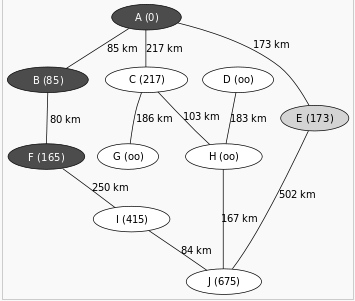
\includegraphics[width=\textwidth]{pics/dijk3.png}
                \caption{Mise à jour et graphe final}
        \end{subfigure}
        \caption{\label{fig:dijkstra}Représentation d'une éxécution de Dijkstra \cite{wikiDijkstra}}
\end{figure}


En effet, le sommet E est rajouté au sous graphe et non le sommet I car la distance à parcourir entre A et E est plus petite que entre A et I.

Il faut souligner que cet algorithme possède le même inconvénient qu'A*.

\begin{subappendices}
  \appsec{Implémentation du déplacement en Lua}
  \subsection{Evitement \emph{greedy}\label{app:implEvitGreedy}}
  \begin{lstlisting}[caption=Initialisation]
function init()
  robot.distance_scanner.enable()
  robot.distance_scanner.set_rpm(SCANNER_RPM)
  obstaclesTable={}
  for i=-PI+PI/DIR_NUMBER, PI-PI/DIR_NUMBER, 2*PI/DIR_NUMBER do
    obstaclesTable[i]=151
  end
  goalX=SOURCEX
  goalY=SOURCEY
end
  \end{lstlisting}
  \begin{lstlisting}[caption=Structure générale]
function step()
  odometry()
  obstaclesTable=updateObstaclesTable(obstaclesTable)
  move(goalX,goalY,obstaclesTable)
end
  \end{lstlisting}
  \begin{lstlisting}[caption=Rafraîchir la table des mesures à chaque pas, label=lst:updateObstaclesTable]
function updateObstaclesTable(tabl, which)
  --tabl: the obstacleTable to refresh
  --(obstaclesTable or shortObstaclesTable)
  --which (string): which sensor to use
  --("short_range" or "long_range")
  local sensor, reading, angle, value, rAngle, rDistance
  for angle, value in pairs(tabl) do
    newValue=false
    for sensor, reading in pairs(robot
                                 .distance_scanner
                                 [which]) do
      rAngle = reading.angle
      rDistance=reading.distance
      if rDistance == -2 then rDistance=151 end
      if rDistance == -1 then rDistance=0 end
      if abs(angle-rAngle)<PI/DIR_NUMBER then
        if value>rDistance or not newValue then
          tabl[angle]=rDistance
          newValue = true
        end
      end
    end
  end
  return tabl
end
  \end{lstlisting}
  \begin{lstlisting}[caption=Fonction move]
function move(goalX,goalY,obstaclesTable)
  local goalDirection=findGoalDirection(posX,posY,goalX,goalY)
  local goalAngle=findGoalAngle(goalDirection, alpha)
  obstacleAvoidance(goalAngle, obstaclesTable)
end
  \end{lstlisting}
  \begin{lstlisting}[caption=Trouver la direction du goal vu du footbot]
function findGoalDirection(posX, posY, goalX, goalY)
  local deltaX=goalX-posX
  local deltaY=goalY-posY
  local goalDirection=math.atan(deltaY/deltaX)
  if deltaX<0 then
    goalDirection=goalDirection+PI
  end
  if goalDirection<0 then
    goalDirection=goalDirection+2*PI
  end
  return goalDirection
end

function findGoalAngle(goalDirection,alpha)
  local goalAngle=goalDirection-alpha
  if goalAngle>PI then
    goalAngle=goalAngle-2*PI
  end
  return goalAngle
end
  \end{lstlisting}
  \begin{lstlisting}[caption=Trouver la direction optimale et la suivre]
function obstacleAvoidance(goalAngle, obstaclesTable)
  local bestAngle, bestDistance, angle, distance
  bestDistance = -1
  for angle, distance in pairs(obstaclesTable) do
    if distance>bestDistance
       or (distance==bestDistance and not bestAngle)
       or (distance==bestDistance
         and abs(angle-goalAngle)<abs(bestAngle-goalAngle)) then
      bestDistance = distance
      bestAngle = angle
    end
  end
  getToGoal(bestAngle, CONVERGENCE)
end
  \end{lstlisting}
  \begin{lstlisting}[caption=Fonction getToGoal]
function getToGoal(angle, conv)
   if angle>=0 then --goal is to the left
      vLeft=speed*((PI-angle)/PI)^conv
      vRight = 2*speed-vLeft
   else --goal is to the right
      vRight=speed*((PI+angle)/PI)^conv
      vLeft = 2*speed - vRight
   end
   robot.wheels.set_velocity(vLeft, vRight)
end
  \end{lstlisting}
  \subsection{Evitement d'obstacles proches \label{app:implEvitClose}}
  \begin{lstlisting}[caption=Capteur supplémentaire]
function step()
  ...
  emerProx, emerDir=readProxSensor()
  if emerProx>0 then
    emergencyAvoidance(emerProx, emerDir)
  else
  ...
end
  \end{lstlisting}
  \begin{lstlisting}[caption=lecture du \emph{proximity sensor}]
function readProxSensor()
  local emerDir = 1
  local emerProx = robot.proximity[1].value
  for i=2,24 do
    if emerProx < robot.proximity[i].value
       or (emerProx == robot.proximity[i].value
           and abs(12-emerDir)<abs(12-i)) then
      emerDir = i
      emerProx = robot.proximity[i].value
    end
  end
  return emerProx, emerDir
end
  \end{lstlisting}

  \begin{lstlisting}[caption=Fonction emergencyAvoidance]
function emergencyAvoidance(emerProx,emerDir)
  local vLeft, vRight
  if emerDir <= 12 then --Obstacle is to the left
    vRight=((1-emerProx)^EMER_PROX_DEP*emerDir
             -EMER_DIR_DEP)
           *speed/11
    vLeft=2*speed-vRight
  else --Obstacle is to the right
    vLeft=((1-emerProx)^EMER_PROX_DEP*(25-emerDir)
            -EMER_DIR_DEP)
          *speed/11
    vRight=2*speed-vLeft
  end
  robot.wheels.set_velocity(vLeft, vRight)
end
  \end{lstlisting}

  \appsec{Ajout d'une composante aléatoire à l'évitement}

\end{subappendices}


\chapter{Recherche du plus court chemin}
\section{Algorithmes déterministes classiques}

Dans le cas où les footbots disposent réellement d'une description complète de leur environnement, il est envisageable d'utiliser les algorithmes classiques de recherche du plus court chemin comme A* et Dijkstra. Ceux-ci fonctionnent en représentant l'environnement sous forme d'un graphe dont les n\oe{}uds représentent les positions accessibles et dont les branches associent à deux n\oe{}uds joignables le coût (ou la distance) qui les sépare. Ces algorithmes associent à un chemin en cours d'évaluation un coût total et sélectionnent au final le chemin au coût le moins élevé.

Dijkstra évalue le coût du chemin courant en calculant simplement la somme des coûts depuis le n\oe{}ud initial. Pour cette raison, il ne privilégie a priori aucune direction d'exploration et son exécution ne se termine que si tous les n\oe{}uds accessibles ont été évalués ou si le n\oe{}ud but a été <<visité>>\footnote{Dans le cas de Dijkstra, <<visité>> signifie que tous les n\oe{}uds adjacents ont été évalués.}.

A* rajoute au coût <<connu>> du chemin reliant l'origine au n\oe{}ud courant l'évaluation heuristique du coût du chemin reliant le point courant au but. Ceci permet de guider la recherche et de l'arrêter plus tôt si on a confiance en l'heuristique utilisée.~\cite{mehlhorn_shortest_2008,genetic2007}

Les algorithmes classiques de recherche du chemin ne sont pas immédiatement adaptables à un environnement partiellement connu ou en cours d'exploration. Des alternatives existent cependant, parmi lesquelles l'utilisation de l'intelligence en essaim, qui s'inspire en partie  des comportements originaux et très efficaces déjà présents dans la nature.

\section{Algorithme des fourmis}

Cet algorithme est basé sur le comportement de certaines colonies de fourmis qui communiquent indirectement par dépôts de phéromones. Il se présente ainsi: lorsqu'une fourmi trouve une source de nourriture, elle dépose, lors de son retour vers la fourmilière, des phéromones tout au long du chemin qu'elle emprunte. Les autres fourmis suivent cette piste de phéromones pour exploiter la source de nourriture et déposent elles aussi des phéromones sur le chemin du retour, qui peut parfois être différent de la piste suivie initialement.

Comme les fourmis suivent préférentiellement les pistes comportant le plus de phéromones, et puisque les phéromones s'évaporent après un certain laps de temps, le chemin le plus court devient rapidement la piste dominante, car plus de fourmis le traversent et déposent des phéromones par unité de temps. De plus, comme les autres pistes sont alors délaissées, cet algorithme converge très fortement car le chemin le plus court devient rapidement l'unique chemin marqué.~\cite{antOpti}

Cette approche a été utilisée par \cite{pheromonesForaging}, ce qui montre qu'il est possible d'appliquer cet algorithme aux footbots dans ARGoS. Ici, ce sont des messages transmis de robot à robot qui jouent le rôle des phéromones, et la rapidité avec laquelle un seule message traverse toute une chaîne de robot qui indique l'<<intensité>> d'une piste; mais les principes fondamentaux restent les mêmes.

\vspace{1em}
Par manque de temps, nous n'avons pas pu implémenter une recherche du chemin efficace en non-omniscient comme ci-dessus, et nous avons choisi de ne pas perdre de temps à implémenter une recherche ``classique'' car elle serait inutile en non-omniscient, qui est le but final du projet.


\chapter[Construction du comportement]{Construction d'un comportement intelligent}
\section{Structure générale \label{sec:stepFunction}}

Après s'être initialisé, chaque footbot éxécute a chaque pas une séquence d'opérations communes à tous les états possibles, suivie d'une séquence s'opérations propre à l'état courant.
\begin{lstlisting}[caption=Fonction step]
function step()
  local obstacleProximity, obstacleDirection, onSource,
        foundSource, backHome, gotSource,
        emerProx, emerDir
  obstacleProximity, obstacleDirection, onSource,
  foundSource, backHome, gotSource,
  emerProx, emerDir = doCommon()
  if emerProx>0 then
    emergencyAvoidance(emerProx, emerDir)
  elseif explore then
    doExplore(obstacleProximity, obstacleDirection,
              foundSource, gotSource)
  else
    doMine(obstacleProximity, obstacleDirection,
           onSource, backHome, foundSource)
  end
end
\end{lstlisting}

\subsection{Opérations Communes}

Les opérations communes à tous les états sont
\begin{itemize}
  \item L'écoute des capteurs <<vitaux>> c'est-à-dire qu'ils peuvent complètement écraser l'état courant: capteur de proximité (déclenche l'évitement d'urgence) et batterie (force le footbot à rentrer au nid)
  \item L'écoute des autres capteurs qui par essence doivent toujours être consultés: capteur de position, de couleur du sol (permet au footbot d'enregistrer des nouvelles sources à tout moment) et communication entre robots (idem).
  \item Lecture du capteur \emph{distance scanner (short range)} parce qu'il est utilisé en pratique quel que soit l'état du robot.
\end{itemize}

L'implémentation détaillée de la fonction doCommon est donnée dans l'annexe \ref{appsec:doCommon}. L'évitement d'urgence est celui présenté dans la section \ref{sec:emerAvoid}, tandis que pour retourner le plus rapidement possible au nid, le footbot utilise simplement le déplacement présenté au chapitre \ref{chap:move} avec pour goal le centre du nid.

\section{Exploration}




\section{Gestion de l'autonomie}
Une condition sur l'autonomie des robots a été imposée: l'autonomie est fixée dans le temps, ce qui signifie que leur batterie se décharge de manière constante à chaque pas d'ARGoS. Une valeur chiffrée n'a pas été imposée, mais les robots doivent juste être capables d'effectuer un aller-retour vers un point le plus éloigné de leur nid de départ à leur vitesse de régime. Une fois la batterie écoulée, le robot est rendu incapable de se déplacer mais pourra peut-être être dépanné par un autre membre de l'essaim dans le futur.

Puisque pour le moment le seul but d'un robot est d'exploiter une ressource, celui-ci peut avorter un aller retour dès qu'il estime qu'il n'est plus capable d'atteindre son but et de revenir ensuite à son nid.

\begin{algorithm}                    
\caption{Battery handling}
\label{algo:batterie}
\begin{algorithmic}[1]
  \REQUIRE \(0 \leq battery \leq 100 :=\) the battery left of the robot
  \ENSURE footbot tries to get back to nest when current goal judged not safely reachable
  \WHILE{goal not reached}
    \STATE update footbot position and battery
    \STATE \(cost \leftarrow evaluate\;cost(position,\;goal,\;[battery])\) \COMMENT{The cost of what is left to do}
    \IF{\(cost > battery\)}
      \STATE \(goal \leftarrow nest\) \COMMENT{Get back to the nest. If the footbot is already on its way back, this doesn't do anything. Appropriate to try to get to the nest when you know you don't have enough to get there?}
    \ENDIF
  \ENDWHILE
\end{algorithmic}
\end{algorithm}
Où evaluate cost(position, goal, [battery]) est la fonction qui évalue l'énergie nécessaire à l'accomplissement du reste du trajet. On peut par exemple utiliser la distance à vol d'oiseau restante à parcourir accompagnée d'un facteur de sécurité, ou alors utiliser une approche heuristique utilisant le rapport entre la batterie utilisée jusqu'au step courant et le déplacement net parcouru vers le but.

En vue de la prochaine étape (la non omniscience des robots), le choix d'implémentation de la batterie autorise des sacrifices, c'est à dire, si un robot, étant à une position, estime devoir aller à une autre position et si sa batterie le lui permet, il ira à cette nouvelle position, sans toutefois vérifier qu'en y allant il pourra rentrer à la base recharger sa batterie. Ce choix favorise l'exploration de l'arène en mettant en avant la réussite de l'ensemble du groupe et non la réussite personnelle, pouvant être interprété comme la recharge de la batterie. Cependant des modifications doivent encore être apportées car nous ne pouvons nous permettre de sacrifier l'ensemble des robots, faute de quoi l'objectif ne sera pas atteint.

\begin{subappendices}
  \appsec{Implémentation de doCommon \label{appsec:doCommon}}
\begin{lstlisting}[caption=fonction doCommon]
function doCommon()
  local obstacleProximity, obstacleDirection,
        onSource, foundSource, backHome, gotSource,
        emerProx, emerDir
  
  odometry()
  onSource, foundSource, backHome = checkGoalReached()
  gotSource = listen()
  shortObstaclesTable = updateObstaclesTable("short_range",
                                             shortObstaclesTable)
  obstacleProximity, obstacleDirection
  =closestObstacleDirection(shortObstaclesTable)

  battery=battery-BATT_BY_STEP
  backForBattery = backForBattery 
                   or battery-batterySecurity
                              *BATT_BY_STEP
                              *math.sqrt(posX^2+posY^2)
                              /BASE_SPEED<10

  emerProx, emerDir=readProxSensor()
  if battery==0 then
    BASE_SPEED=0
    logerr("batt empty")
  end
  if currentStep%5000==0 then
    log(travels)
  end
  return obstacleProximity, obstacleDirection,
         onSource, foundSource, backHome,
         gotSource, emerProx, emerDir
end
\end{lstlisting}

\begin{lstlisting}[]

\end{lstlisting}

\end{subappendices}


\chapter{Résultats obtenus}
Le comportement créé permet de remplir tous les objectifs énoncés par le cahier des charges, à savoir l'exploration d'un environnement inconnu dans le but d'y repérer des <<sources>> marquées par des taches noires au sol et l'exploitation de ces sources, tout en évitant les obstacles éventuels et en gérant adéquatement l'autonomie des robots. De plus, l'arène a aussi dû être créée afin de convenir à l'expérience ainsi qu'aux spécifications données. Enfin, comme demandé, une évaluation des performances du comportement a été faite. Cette évaluation est présentée ci-dessous.

\section{Evaluation des performances}

Etude statistique encore en cours

\section{Perspectives d'amélioration}

\subsection{Optimisation des constantes utilisées}
Tout au long de ce rapport, différents paramètres numériques ont été mis en avant et le comportement Lua a aussi été écrit de manière à ce que ces valeurs soient facilement accessibles. Il en résulte un ensemble de variables globales qui régissent toutes un aspect du comportement du robot dans l'expérience.

\begin{lstlisting}[caption=Définitions des variables globales]
--Specs received
BASE_SPEED=30
BATT_BY_STEP =.2

--Low-level
SCANNER_RPM=75
DIR_NUMBER = 15
EXPL_DIR_NUMBER = 20
EXPL_CONV = 3

--"Mid"-level:Movement
CONVERGENCE=1
OBSTACLE_PROXIMITY_DEPENDANCE=.25
OBSTACLE_DIRECTION_DEPENDANCE=.25
EMER_DIR_DEP=1
EMER_PROX_DEP=1
MIN_SPEED_COEFF = 0.6
--When a footbot "hits" something, he will pick a
--temporary speed between this coeff and 1 times BASE_SPEED
RANDOM_SPEED_TIME = 30
--The number of steps during which
--the footbot keeps this new random speed

--High-level:Decision Making
ORGN_SRC_DST=80
--Minimal distance between two sources considered "different"
MINE_PROB_WHEN_SRC_RECVD=.2
--Probability of starting mining upon receiving a new source
INIT_BATT_SEC=25
--Initial battery handling security coeff
IDEAL_NEST_BATT=20
--Leftover battery a footbot should have when returning to the nest
EPSILONGREED=0.1
--epsilon for epsilon-greedy choice algorithm
\end{lstlisting}

L'étape suivante consisterait à trouver une combinaison de ces variables qui maximise la performance des robots. Ceci est bien évidemment une problématique très vaste, d'une part parce que cette combinaison optimale de valeurs dépend de la manière dont la performance est mesurée et de la configuration d'expérience utilisée, et d'autre part parce que le nombre de ces variables est trop déraisonnablement élevé pour se lancer dans une telle optimisation sans d'abord essayer de simplifier le problème. Dans cette section, nous allons brièvement rappeler les paramètres qui sont apparus, montrer quelles sont les constantes qui jouent les rôles les plus importants et quelles possibilités immédiates d'adaptation notre comportement offre à travers la modification de ces variables globales.

Les constantes sont réparties en trois groupes: les constantes <<bas-niveau>>, les constantes utilisées par les différents algorithmes de déplacement, et les constantes <<haut-niveau>> qui interviennent dans la prise de décision. Parmi les constantes <<bas-niveau>>, on trouve la vitesse angulaire du \emph{distance scanner}, le nombre de directions dans lesquelles les mesures de ce capteur sont regroupées ainsi que la convergence $\kappa$ utilisée pour les <<rebonds>> lors de l'exploration\footnote{voir listing \ref{list:gaslike}.}. Ces constantes jouent un rôle extrèmement mineur et sont plutôt liées à la physique des footbots.

Dans les constantes liées au mouvement, on retrouve la convergence $\kappa$ utilisée dans le reste des situations ainsi que les deux paires de paramètres $\alpha$ et $\beta$ qui sont apparus dans l'évitement d'obstacles proches en \ref{sec:emerAvoid} et l'évitement intermédiaire en \ref{sec:mediAvoid}\footnote{Pour rappel, ces deux évitements sont les mêmes aux constantes et à la portée des capteurs utilisés près}. On retrouve aussi les paramètres utilisés pour introduire une composante aléatoire à l'évitement dans l'annexe \ref{appsec:randomAvoidance}. Ces constantes influent sur la qualité générale du mouvement à travers toute l'expérience, et il existe probablement une plage de valeurs qui optimisent le mouvement dans l'écrasante majorité des configurations. En d'autres termes, elles ne permettent pas d'adapter le comportement des footbots d'une situation a une autre.

Dans les constantes <<haut niveau>> liées à la prise de décision, on retrouve la distance minimale entre deux sources pour qu'elles soient considérées comme originales, la probabilité qu'un footbot commence à miner les ressources qu'il connaît lorsqu'il reçoit une nouvelle source, le coefficient de sécurité initial utilisé dans la gestion de l'autonomie, le résidu de batterie idéal que doit avoir le robot lorsqu'il rentre au nid pour se ravitailler, ainsi que la valeur du $\varepsilon$ utilisé dans la décision $\varepsilon$-greedy. Ces variables ont elles une influence majeure sur le comportement final des robots. Tout travail d'optimisation ultérieur devrait se pencher en priorité sur ces constantes-ci.

Parmi ces variables, il est cependant possible de mettre {\ttfamily INIT\_BATT\_SEC} à part car comme son nom l'indique il ne s'agit que du coefficient de sécurité initial puisqu'il est ensuite réévalué constamment durant l'expérience. Il suffit donc de lui donner une valeur largement supérieure à la normale et celle-ci sera abaissée au cours de l'éxécution. Pour jouer sur la prise de risque liée à la gestion de la batterie, il faut utiliser {\ttfamily IDEAL\_NEST\_BATT}.

{\ttfamily ORGN\_SRC\_DST} et {\ttfamily MINE\_PROB\_WHEN\_SRC\_RECVD} sont assez étroitement liées. L'influence de {\ttfamily ORGN\_SRC\_DST} est assez claire, mais lorque cette constante est modifiée, il faut penser à modifier {\ttfamily MINE\_PROB\_WHEN\_SRC\_RECVD} en parallèle. En effet, pour un même nombre de sources <<réellement différentes>> abaisser la première de ces constantes augmente le nombre de sources <<différentes selon les robots>> à découvrir et il est donc judicieux d'augmenter par la même occasion la tendance à l'exploration par le biais de {\ttfamily MINE\_PROB\_WHEN\_SRC\_RECVD}. De même, il peut être judicieux de jouer sur cette dernière constante si l'on dispose d'informations sur le nombre de sources réelles ou selon le but de l'expérience: rendement court-terme, rendement long-terme, découverte d'une proportion maximale des ressources,~\ldots\ Cependant, l'importance de ces deux variables peut-être réduite si l'on implémente les deux transitions supplémentaires proposées dans le diagramme \ref{fig:genFlowchart}.

Enfin, l'influence de $\varepsilon$ dans la décision $\varepsilon$-greedy est assez claire et bien documentée (voir par exemple \cite{foraging}.). Etant donné les résultats des études statistiques, une valeur plus élevée que celle utilisée ($0.1$) semble peut-être judicieuse, à moins qu'une refonte totale du choix de la source à exploiter ne soit nécessaire.

\subsection{Amélioration plus fondamentales (??)(This is bad)}

TODO



\chapter{Fonctionnement du groupe}
Le groupe est composé de 5 membres. Chaque membre possède sa manière de travailler, de comprendre, de communiquer. Une des difficultés d’un travail d’équipe est de pouvoir combiner tous ces caractères pour que le projet se déroule dans les meilleures conditions et que chacun puisse trouver sa place. Donc pour comprendre le fonctionnement de chacun, chaque membre a dû présenter ses points forts et ses points faibles. Le but de cette démarche est de pouvoir répartir les tâches au mieux tout en privilégiant le transfert de compétences. Ceci a été fait par exemple lors de la présentation orale formative de mi-parcours, où les membres qui se sentaient le moins à l’aise dans l'exercice ont choisi de faire cette présentation afin de pouvoir profiter de l'opportunité.

\subsubsection{Organisation et communication}

La répartition des tâches se fait spontanément en fonction des besoins pour l’avancée du projet ainsi que des membres qui ont travaillé sur des tâches similaires dans le passé. Ceci offre l’avantage d’une meilleure gestion du temps lors des réunions car les membres sont au courant des problèmes à régler. Cependant un diagramme de Gantt (cf. annexe) a été créé pour aussi avoir une vision plus globale de l’avancement du projet et également se fixer des dates butoir.

A côté des moyens de communication habituellement utilisés tels que l'utilisation de mails et de réseau sociaux, des outils plus spécifiques ont été mis en place afin d'améliorer l'implication des membres et l'efficacité du travail collectif. Tout d'abord, un dépôt git a été créé \footnote{\url{https://github.com/nathdwek/projetBa2} et \url{https://github.com/nathdwek/rapportProjetBa2}} afin de pouvoir profiter de tous les avantages qu'offre un contrôleur de version distribué: sécurité, travail simultané sur plusieurs aspects du code tout en maintenant une version parfaitement fonctionelle, possibilité de consulter l'historique,~\ldots Nous avons essayé de passer systématiquement par l'usage de branches afin de nouveau de gagner en sécurité, ce qui permet à n'importe quel membre d'essayer sans crainte et sans perte de temps d'implémenter une fonctionnalité ou de corriger une erreur éventuelle. D'autre part, nous avons utilisé Zotero pour la mise en commun, l'uniformisation et l'export en format Bibtex des ressources bibliographiques.

\begin{figure}[htb]
  \centering
  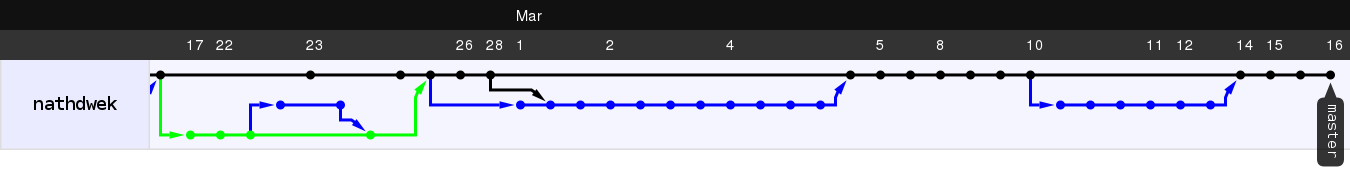
\includegraphics[width=\textwidth]{pics/workflow.png}
    \caption{Réseau de commits récents du projet}
\end{figure}


\listofalgorithms

\addcontentsline{toc}{chapter}{Table des algorithmes}

\lstlistoflistings

\addcontentsline{toc}{chapter}{Table des listings}

\listoffigures

\addcontentsline{toc}{chapter}{Table des figures}

\nocite{*}

\bibliography{rapport}

\addcontentsline{toc}{chapter}{\bibname}

\end{document}
